% Options for packages loaded elsewhere
% Options for packages loaded elsewhere
\PassOptionsToPackage{unicode}{hyperref}
\PassOptionsToPackage{hyphens}{url}
%
\documentclass[
  ignorenonframetext,
  aspectratio=169,
]{beamer}
\newif\ifbibliography
\usepackage{pgfpages}
\setbeamertemplate{caption}[numbered]
\setbeamertemplate{caption label separator}{: }
\setbeamercolor{caption name}{fg=normal text.fg}
\beamertemplatenavigationsymbolsempty
% remove section numbering
\setbeamertemplate{part page}{
  \centering
  \begin{beamercolorbox}[sep=16pt,center]{part title}
    \usebeamerfont{part title}\insertpart\par
  \end{beamercolorbox}
}
\setbeamertemplate{section page}{
  \centering
  \begin{beamercolorbox}[sep=12pt,center]{section title}
    \usebeamerfont{section title}\insertsection\par
  \end{beamercolorbox}
}
\setbeamertemplate{subsection page}{
  \centering
  \begin{beamercolorbox}[sep=8pt,center]{subsection title}
    \usebeamerfont{subsection title}\insertsubsection\par
  \end{beamercolorbox}
}
% Prevent slide breaks in the middle of a paragraph
\widowpenalties 1 10000
\raggedbottom
\usepackage{iftex}
\ifPDFTeX
  \usepackage[T1]{fontenc}
  \usepackage[utf8]{inputenc}
  \usepackage{textcomp} % provide euro and other symbols
\else % if luatex or xetex
  \usepackage{unicode-math} % this also loads fontspec
  \defaultfontfeatures{Scale=MatchLowercase}
  \defaultfontfeatures[\rmfamily]{Ligatures=TeX,Scale=1}
\fi
\usepackage{lmodern}

\ifPDFTeX\else
  % xetex/luatex font selection
\fi
% Use upquote if available, for straight quotes in verbatim environments
\IfFileExists{upquote.sty}{\usepackage{upquote}}{}
\IfFileExists{microtype.sty}{% use microtype if available
  \usepackage[]{microtype}
  \UseMicrotypeSet[protrusion]{basicmath} % disable protrusion for tt fonts
}{}
\makeatletter
\@ifundefined{KOMAClassName}{% if non-KOMA class
  \IfFileExists{parskip.sty}{%
    \usepackage{parskip}
  }{% else
    \setlength{\parindent}{0pt}
    \setlength{\parskip}{6pt plus 2pt minus 1pt}}
}{% if KOMA class
  \KOMAoptions{parskip=half}}
\makeatother


\usepackage{longtable,booktabs,array}
\usepackage{calc} % for calculating minipage widths
\usepackage{caption}
% Make caption package work with longtable
\makeatletter
\def\fnum@table{\tablename~\thetable}
\makeatother
\usepackage{graphicx}
\makeatletter
\newsavebox\pandoc@box
\newcommand*\pandocbounded[1]{% scales image to fit in text height/width
  \sbox\pandoc@box{#1}%
  \Gscale@div\@tempa{\textheight}{\dimexpr\ht\pandoc@box+\dp\pandoc@box\relax}%
  \Gscale@div\@tempb{\linewidth}{\wd\pandoc@box}%
  \ifdim\@tempb\p@<\@tempa\p@\let\@tempa\@tempb\fi% select the smaller of both
  \ifdim\@tempa\p@<\p@\scalebox{\@tempa}{\usebox\pandoc@box}%
  \else\usebox{\pandoc@box}%
  \fi%
}
% Set default figure placement to htbp
\def\fps@figure{htbp}
\makeatother





\setlength{\emergencystretch}{3em} % prevent overfull lines

\providecommand{\tightlist}{%
  \setlength{\itemsep}{0pt}\setlength{\parskip}{0pt}}



 


% ============================================================
%  ECO 2203 — Beamer Metropolis Theme Preamble
%  Course: International Trade and Policy in Agriculture
%  Instructor: Nithin M, Department of Development Economics
% ============================================================

% MUST be first: load Metropolis theme before \metroset and colour overrides
\usetheme{metropolis}

% Only load packages not already provided by pandoc's beamer template
\usepackage{amsmath,amssymb}

% ---- Brand colours -----------------------------------------
\definecolor{brandblue}{HTML}{012169}
\definecolor{brandgold}{HTML}{B9975B}
\definecolor{lightblue}{HTML}{E8EDF5}

% ---- Metropolis colour overrides ---------------------------
% Main palette
\setbeamercolor{normal text}{fg=black,bg=white}
\setbeamercolor{alerted text}{fg=brandgold}
\setbeamercolor{example text}{fg=brandblue!70!black}

% Title slide
\setbeamercolor{title}{fg=white,bg=brandblue}
\setbeamercolor{subtitle}{fg=brandgold}
\setbeamercolor{author}{fg=white}
\setbeamercolor{institute}{fg=brandgold!80!white}
\setbeamercolor{date}{fg=white}
\setbeamercolor{title page header}{fg=white,bg=brandblue}

% Frametitle bar
\setbeamercolor{frametitle}{fg=white,bg=brandblue}

% Progress bar → gold
\setbeamercolor{progress bar}{fg=brandgold,bg=brandblue!30}
\setbeamercolor{title separator}{fg=brandgold}
\setbeamercolor{progress bar in head/foot}{fg=brandgold,bg=brandblue!20}
\setbeamercolor{progress bar in section page}{fg=brandgold,bg=brandblue!20}

% Blocks
\setbeamercolor{block title}{bg=brandblue,fg=white}
\setbeamercolor{block body}{bg=lightblue,fg=black}
\setbeamercolor{block title alerted}{bg=brandgold,fg=white}
\setbeamercolor{block body alerted}{bg=brandgold!12,fg=black}
\setbeamercolor{block title example}{bg=brandblue!70!black,fg=white}
\setbeamercolor{block body example}{bg=brandblue!8,fg=black}

% Structure / lists
\setbeamercolor{structure}{fg=brandblue}
\setbeamercolor{section in toc}{fg=brandblue}
\setbeamercolor{itemize item}{fg=brandblue}
\setbeamercolor{itemize subitem}{fg=brandgold}
\setbeamercolor{enumerate item}{fg=brandblue}
\setbeamercolor{description item}{fg=brandblue}

% ---- Metropolis options ------------------------------------
\metroset{
  progressbar    = frametitle,   % gold bar under frametitle
  sectionpage    = none,
  numbering      = fraction,
  block          = fill
}

% ---- Fonts (Metropolis uses Fira Sans; fallback gracefully) -
\setbeamerfont{title}{size=\Large,series=\bfseries}
\setbeamerfont{subtitle}{size=\normalsize,series=\mdseries}
\setbeamerfont{frametitle}{size=\large,series=\bfseries}
\setbeamerfont{block title}{size=\normalsize,series=\bfseries}
\setbeamerfont{caption}{size=\footnotesize}

% ---- Footer: course info + slide number --------------------
\setbeamertemplate{footline}{%
  \begin{beamercolorbox}[wd=\paperwidth,ht=2.0ex,dp=1ex]{footline}%
    \hspace{0.8em}%
    {\footnotesize\color{brandblue!60}%
      ECO 2203 \textbar{} International Trade and Policy in Agriculture
      \hfill Nithin M \hfill
      \insertframenumber{}/\inserttotalframenumber\hspace{0.8em}}%
  \end{beamercolorbox}%
}

% ---- Misc --------------------------------------------------
\setlength{\parskip}{0.25em}
\setbeamertemplate{navigation symbols}{}

% tighter column sep for side-by-side content
\setlength{\columnsep}{0.8em}

% Fix: make \label truly robust in moving arguments (Quarto generates
% \caption{\label{fig-xxx}...} which crashes Metropolis in batchmode).
% DeclareRobustCommand creates a self-protecting robust version.
\makeatletter
\let\quarto@originallabel\label
\DeclareRobustCommand*{\label}[1]{\quarto@originallabel{#1}}
\makeatother

% Prevent figures from overflowing Beamer frames.
% width=\linewidth: scale to text width (already Quarto default);
% height=0.6\textheight: cap height so figures never push past the frame bottom.
% keepaspectratio: never distort — whichever constraint binds first wins.
\setkeys{Gin}{width=\linewidth,height=0.6\textheight,keepaspectratio}
\makeatletter
\@ifpackageloaded{caption}{}{\usepackage{caption}}
\AtBeginDocument{%
\ifdefined\contentsname
  \renewcommand*\contentsname{Table of contents}
\else
  \newcommand\contentsname{Table of contents}
\fi
\ifdefined\listfigurename
  \renewcommand*\listfigurename{List of Figures}
\else
  \newcommand\listfigurename{List of Figures}
\fi
\ifdefined\listtablename
  \renewcommand*\listtablename{List of Tables}
\else
  \newcommand\listtablename{List of Tables}
\fi
\ifdefined\figurename
  \renewcommand*\figurename{Figure}
\else
  \newcommand\figurename{Figure}
\fi
\ifdefined\tablename
  \renewcommand*\tablename{Table}
\else
  \newcommand\tablename{Table}
\fi
}
\@ifpackageloaded{float}{}{\usepackage{float}}
\floatstyle{ruled}
\@ifundefined{c@chapter}{\newfloat{codelisting}{h}{lop}}{\newfloat{codelisting}{h}{lop}[chapter]}
\floatname{codelisting}{Listing}
\newcommand*\listoflistings{\listof{codelisting}{List of Listings}}
\makeatother
\makeatletter
\makeatother
\makeatletter
\@ifpackageloaded{caption}{}{\usepackage{caption}}
\@ifpackageloaded{subcaption}{}{\usepackage{subcaption}}
\makeatother

\usepackage{bookmark}
\IfFileExists{xurl.sty}{\usepackage{xurl}}{} % add URL line breaks if available
\urlstyle{same}
\hypersetup{
  pdftitle={Lecture 16: Export Procedures and Documentation},
  pdfauthor={Nithin M},
  hidelinks,
  pdfcreator={LaTeX via pandoc}}


\title{Lecture 16: Export Procedures and Documentation}
\subtitle{ECO 2203 \textbar{} International Trade and Policy in
Agriculture}
\author{Nithin M}
\date{2026-08-08}
\institute{Department of Development Economics}

\begin{document}
\frame{\titlepage}


\begin{frame}{}
\phantomsection\label{section}
\textbf{Lecture 16}

{Export Procedures and Documentation}

From Karnataka Farm to Leicester Kitchen
\end{frame}

\begin{frame}
\begin{block}{Opening: The Journey of a Kilo of Tur Dal}
\phantomsection\label{opening-the-journey-of-a-kilo-of-tur-dal}
\begin{columns}[T]
\begin{column}{0.58\linewidth}
A kilo of \textbf{Kalaburagi tur dal} travels from a Karnataka farmer to
a diaspora kitchen in \textbf{Leicester, UK}.

What stands between the farmer and the foreign consumer?

\begin{itemize}
\tightlist
\item
  Registrations with four government agencies
\item
  Twelve documents crossing seven desks
\item
  Two financial instruments spanning two continents
\item
  One customs portal used by 1.4 million exporters
\end{itemize}

\textbf{Today's lecture answers: how does this actually work?}
\end{column}

\begin{column}{0.42\linewidth}
\textbf{India's agri export snapshot (FY2024):}

\begin{itemize}
\tightlist
\item
  Total agri exports: \textbf{₹3.61 lakh crore (\textasciitilde\$43.7B)}
\item
  Agricultural exporters registered: \textbf{\textasciitilde85,000}
\item
  Ports handling agri cargo: \textbf{13 major + 200 minor}
\item
  Average documents per shipment: \textbf{8--12}
\end{itemize}

Every export begins with a registration and ends with a bank
certificate.
\end{column}
\end{columns}
\end{block}
\end{frame}

\begin{frame}
\begin{block}{Step 1 --- Pre-Export Registrations: The Four Pillars}
\phantomsection\label{step-1-pre-export-registrations-the-four-pillars}
\begin{columns}[T]
\begin{column}{0.55\linewidth}
Before any shipment, an agricultural exporter must hold:

\textbf{1. Import Export Code (IEC)} - Issued by DGFT (Director General
of Foreign Trade) - 10-digit PAN-based code --- \textbf{mandatory} for
all exports - One-time registration; lifelong validity - Apply online at
dgft.gov.in --- fee ₹500

\textbf{2. RCMC (Registration-cum-Membership Certificate)} - Issued by
the relevant commodity body: - {APEDA} --- processed food, fresh
produce, meat, dairy, cereals - {MPEDA} --- marine products - {Spices
Board} --- all spices - {Coffee/Tea/Rubber Board} --- respective
commodities
\end{column}

\begin{column}{0.45\linewidth}
\textbf{3. GST Registration}

GSTIN is mandatory for tax input credit on export supplies. Exports are
\textbf{zero-rated} under GST --- exporter can claim refund of input
taxes.

\textbf{4. AD Bank Account}

Authorised Dealer (AD) Category-I bank account for receiving foreign
exchange. FEMA requires all export proceeds to be realised through an AD
bank within \textbf{9 months} of shipment.
\end{column}
\end{columns}

\textbf{Sequence matters:} IEC → GST → RCMC → AD Bank account. No RCMC
without IEC. No export incentive claim without RCMC.
\end{block}
\end{frame}

\begin{frame}
\begin{block}{Export Contracts and Incoterms 2020}
\phantomsection\label{export-contracts-and-incoterms-2020}
\begin{columns}[T]
\begin{column}{0.55\linewidth}
An \textbf{export contract} specifies: price, quantity, quality,
delivery terms, payment mode, and dispute resolution.

\textbf{Incoterms 2020} (ICC, Paris) --- 11 standardised trade terms
that define exactly \textbf{where risk and cost transfer} from seller to
buyer.

Key terms for Indian agri exports:

\begin{longtable}[]{@{}lll@{}}
\toprule\noalign{}
Term & Risk Transfers At & Used For \\
\midrule\noalign{}
\endhead
{EXW} & Seller's premises & Rare in agri \\
{FCA} & Named place to carrier & Air/rail shipments \\
{FOB} & On board vessel & \textbf{Most Indian agri} \\
{CIF} & Destination port & Buyer-preferred \\
{DDP} & Buyer's premises & E-commerce niche \\
\bottomrule\noalign{}
\end{longtable}
\end{column}

\begin{column}{0.45\linewidth}
\textbf{FOB vs CIF for India:}

Under \textbf{FOB}, the Indian exporter's responsibility ends when goods
cross the ship's rail. Freight and insurance arranged by the buyer.

Under \textbf{CIF}, the exporter arranges (and prices) freight and
insurance to the destination port.

\textbf{\textasciitilde65\% of India's agri exports are on FOB terms.}
CIF is preferred by Gulf and African buyers who have captive freight
arrangements.

\textbf{Negotiation tip:} FOB is simpler for small exporters; CIF offers
a higher invoice value and more price control.
\end{column}
\end{columns}
\end{block}
\end{frame}

\begin{frame}
\begin{block}{Export Documents: Proof of Transaction}
\phantomsection\label{export-documents-proof-of-transaction}
\begin{columns}[T]
\begin{column}{0.5\linewidth}
\begin{enumerate}
\tightlist
\item
  \textbf{Commercial Invoice} --- price, quantity, HSN code, IEC,
  buyer/seller details; basis for customs valuation
\item
  \textbf{Packing List} --- box-by-box itemisation of weight,
  dimensions, marks
\item
  \textbf{Bill of Lading (B/L)} --- title document issued by shipping
  line; original B/L needed to claim cargo
\item
  \textbf{Airway Bill (AWB)} --- air freight equivalent of B/L;
  non-negotiable consignment note
\item
  \textbf{Certificate of Origin (CoO)} --- issued by FIEO/chamber;
  determines FTA preferential tariff eligibility
\end{enumerate}
\end{column}

\begin{column}{0.5\linewidth}
The \textbf{Bill of Lading} is the only document that is a negotiable
instrument --- it can be endorsed and transferred like a cheque.
\end{column}
\end{columns}

\note{Detailed descriptions:

\begin{enumerate}
\tightlist
\item
  \textbf{Commercial Invoice} --- price, quantity, HSN code, IEC,
  buyer/seller details; basis for customs valuation and bank payment
  verification under LC.
\item
  \textbf{Packing List} --- box-by-box itemisation of weight,
  dimensions, marks and numbers; used by customs and buyer for checking
  receipt.
\item
  \textbf{Bill of Lading (B/L)} --- shipping company's receipt and title
  document; original needed to claim cargo at destination port;
  negotiable instrument that can be endorsed and transferred.
\item
  \textbf{Airway Bill (AWB)} --- non-negotiable air freight equivalent
  of B/L; issued by airline; consignee named directly.
\item
  \textbf{Certificate of Origin (CoO)} --- issued by FIEO, chamber of
  commerce, or APEDA; proves country of origin; required for
  preferential duty rate under FTAs.
\end{enumerate}}
\end{block}

\begin{block}{Export Documents: Compliance and Regulatory}
\phantomsection\label{export-documents-compliance-and-regulatory}
\begin{columns}[T]
\begin{column}{0.5\linewidth}
\begin{enumerate}
\setcounter{enumi}{5}
\tightlist
\item
  \textbf{Phytosanitary Certificate} --- issued by PPQS (Plant
  Protection, Quarantine \& Storage); mandatory for all plant products
\item
  \textbf{Health / Inspection Certificate} --- issued by EIC for meat,
  marine, organic, dairy exports
\item
  \textbf{EDPMS declaration} --- RBI's online system linking shipment to
  forex realization
\item
  \textbf{Fumigation Certificate} --- mandatory for pulses, oilseeds;
  issued by certified fumigators
\item
  \textbf{Shipping Bill} --- key customs clearance document filed on
  ICEGATE; must be approved before loading
\end{enumerate}
\end{column}

\begin{column}{0.5\linewidth}
\textbf{Document flow for a typical agri export:}

\begin{enumerate}
\tightlist
\item
  Export contract signed → Commercial Invoice prepared
\item
  LC opened by buyer's bank
\item
  Shipment arranged → B/L issued
\item
  Phytosanitary + Fumigation certificates obtained
\item
  Shipping Bill filed on ICEGATE → LEO (Let Export Order) obtained
\item
  Documents presented to advising bank → payment
\item
  EDPMS updated → forex realization confirmed
\end{enumerate}
\end{column}
\end{columns}

\note{Detailed descriptions:

\begin{enumerate}
\setcounter{enumi}{5}
\tightlist
\item
  \textbf{Phytosanitary Certificate} --- issued by Directorate of Plant
  Protection, Quarantine \& Storage (PPQS) under DAPFW; certifies
  products are pest-free; mandatory for all plant and plant-product
  exports.
\item
  \textbf{Health / Inspection Certificate} --- issued by Export
  Inspection Council (EIC) for meat, marine, organic, and dairy exports;
  confirms product meets importing country food safety standards.
\item
  \textbf{EDPMS declaration} (Export Data Processing and Monitoring
  System) --- RBI's online system; all export shipments must be
  registered; links shipment data to forex realization within 9 months.
\item
  \textbf{Fumigation Certificate} --- mandatory for pulses, oilseeds,
  and many cereals; issued by certified fumigators; many countries
  require methyl bromide or phosphine treatment; certificate must
  specify chemical, dosage, duration.
\item
  \textbf{Shipping Bill} --- the key customs clearance document filed on
  ICEGATE; must be approved by Customs before loading; distinct types
  (Free Shipping Bill, Dutiable SB, SB under claim for Drawback) for
  different incentive claims.
\end{enumerate}}
\end{block}
\end{frame}

\begin{frame}
\begin{block}{Letter of Credit: Reducing Counterparty Risk}
\phantomsection\label{letter-of-credit-reducing-counterparty-risk}
\begin{columns}[T]
\begin{column}{0.55\linewidth}
\textbf{Why LC?} In international trade, buyer and seller do not know
each other. The LC inserts two banks as guarantors.

\textbf{Step-by-step LC mechanism:}

\begin{enumerate}
\tightlist
\item
  Buyer and seller agree on price and LC terms
\item
  \textbf{Buyer's bank (Issuing Bank)} issues LC in favour of exporter
\item
  \textbf{Advising Bank} (exporter's bank in India) notifies exporter;
  may also confirm
\item
  Exporter ships goods; presents documents to advising bank
\item
  Documents checked against LC terms; bank pays exporter
\item
  Documents forwarded to issuing bank; buyer pays and gets documents
\item
  Buyer presents B/L to shipping line → collects cargo
\end{enumerate}
\end{column}

\begin{column}{0.45\linewidth}
\textbf{Types of LC:}

\begin{itemize}
\tightlist
\item
  \textbf{Sight LC:} Exporter paid immediately on document presentation
\item
  \textbf{Usance/DA LC:} Payment deferred (30, 60, 90 days) --- extends
  credit to buyer
\item
  \textbf{Revolving LC:} Renews automatically for repeat shipments
\item
  \textbf{Back-to-Back LC:} Small exporters use master LC as collateral
  to open LC for their suppliers
\end{itemize}

\textbf{India's EXIM Bank:} Pre-shipment and post-shipment credit;
refinances AD banks for agri exporters.

\textbf{ECGC:} Export Credit Guarantee Corporation --- insures against
buyer default and country risk. Premium: \textasciitilde0.5--1\% of
invoice value.
\end{column}
\end{columns}
\end{block}
\end{frame}

\begin{frame}
\begin{block}{Export Credit: Pre vs Post Shipment Trend}
\phantomsection\label{export-credit-pre-vs-post-shipment-trend}
\begin{figure}

\centering{

\pandocbounded{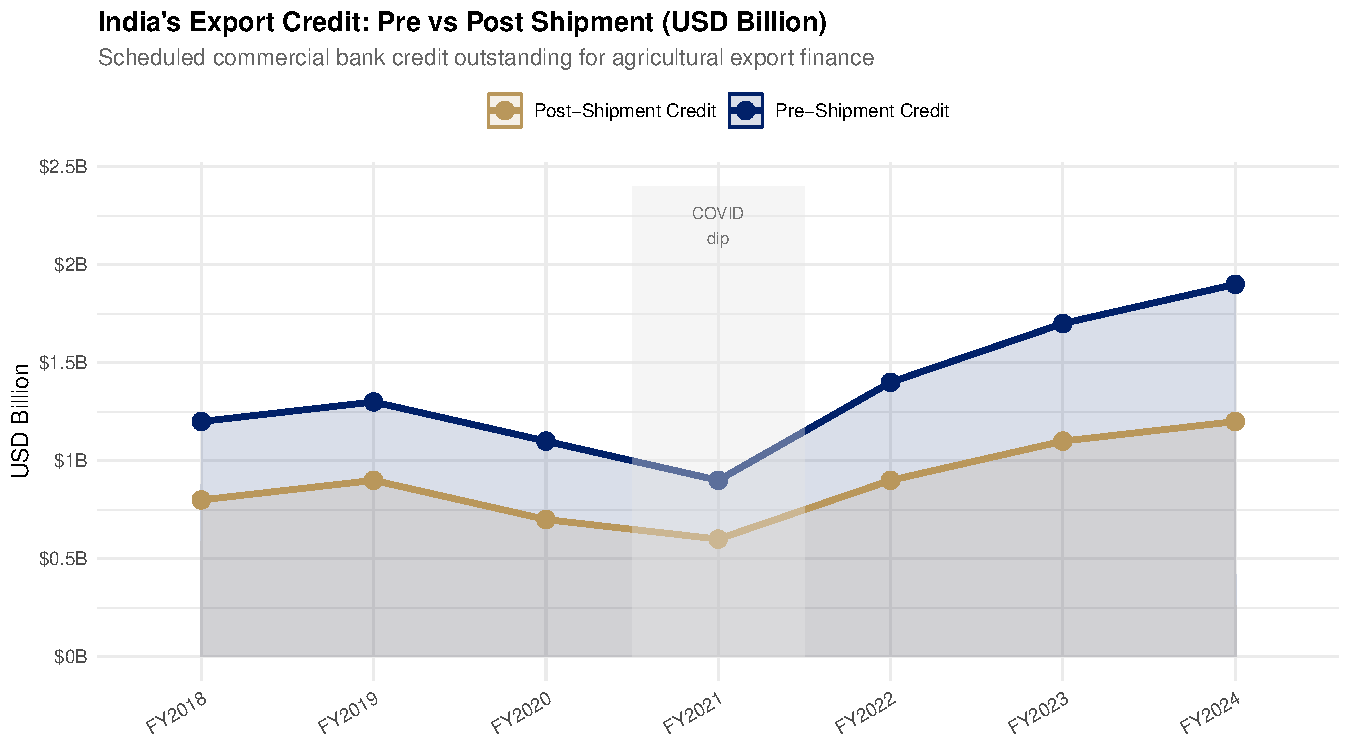
\includegraphics[keepaspectratio]{Lecture16_Export_Procedures_files/figure-beamer/fig-export-credit-1.pdf}}

}

\caption{\label{fig-export-credit}Pre-shipment credit dipped during
COVID (FY2021) and recovered alongside export growth; post-shipment
credit tracks pre-shipment with a structural lag. Source: RBI, Handbook
of Statistics on Indian Economy.}

\end{figure}%
\end{block}
\end{frame}

\begin{frame}
\begin{block}{Customs Clearance: ICEGATE and the Shipping Bill}
\phantomsection\label{customs-clearance-icegate-and-the-shipping-bill}
\begin{columns}[T]
\begin{column}{0.55\linewidth}
\textbf{ICEGATE} (Indian Customs EDI Gateway) --- the single portal for
all Indian customs transactions.

\textbf{Shipping Bill types:}

\begin{longtable}[]{@{}ll@{}}
\toprule\noalign{}
Type & When Used \\
\midrule\noalign{}
\endhead
\textbf{Drawback SB} & Claiming duty drawback on inputs \\
\textbf{DEEC/Advance Auth SB} & Against advance authorisation \\
\textbf{EP Copy SB} & Ordinary exports \\
\textbf{Free Shipping Bill} & Personal effects, gifts \\
\bottomrule\noalign{}
\end{longtable}

\textbf{Process flow:} 1. Exporter files Shipping Bill online with all
document details 2. Customs Risk Management System (RMS) assesses risk
3. Low-risk: \textbf{Green Channel} → LEO (Let Export Order) in 2--4
hours 4. Medium-risk: \textbf{Yellow Channel} → document examination 5.
High-risk: \textbf{Red Channel} → physical examination of cargo
\end{column}

\begin{column}{0.45\linewidth}
\textbf{LEO --- Let Export Order:}

The LEO is the customs officer's green light for loading. Cargo
\textbf{cannot board} without LEO. Once LEO is given:

\begin{itemize}
\tightlist
\item
  Exporter has 24 hours to load at port
\item
  Date of LEO = official date of export for FEMA and incentive purposes
\end{itemize}

\textbf{AEO Status (Authorised Economic Operator):}

Exporters with strong compliance history can apply for AEO status (Tier
I, II, III). Benefits: - Fast-track customs clearance - Reduced physical
examination - Priority in port queue - Deferred duty payment

In FY2024, \textasciitilde12,000 entities hold AEO status in India.
\end{column}
\end{columns}
\end{block}
\end{frame}

\begin{frame}
\begin{block}{India's Merchandise Exports by Mode of Transport}
\phantomsection\label{indias-merchandise-exports-by-mode-of-transport}
\begin{figure}

\centering{

\pandocbounded{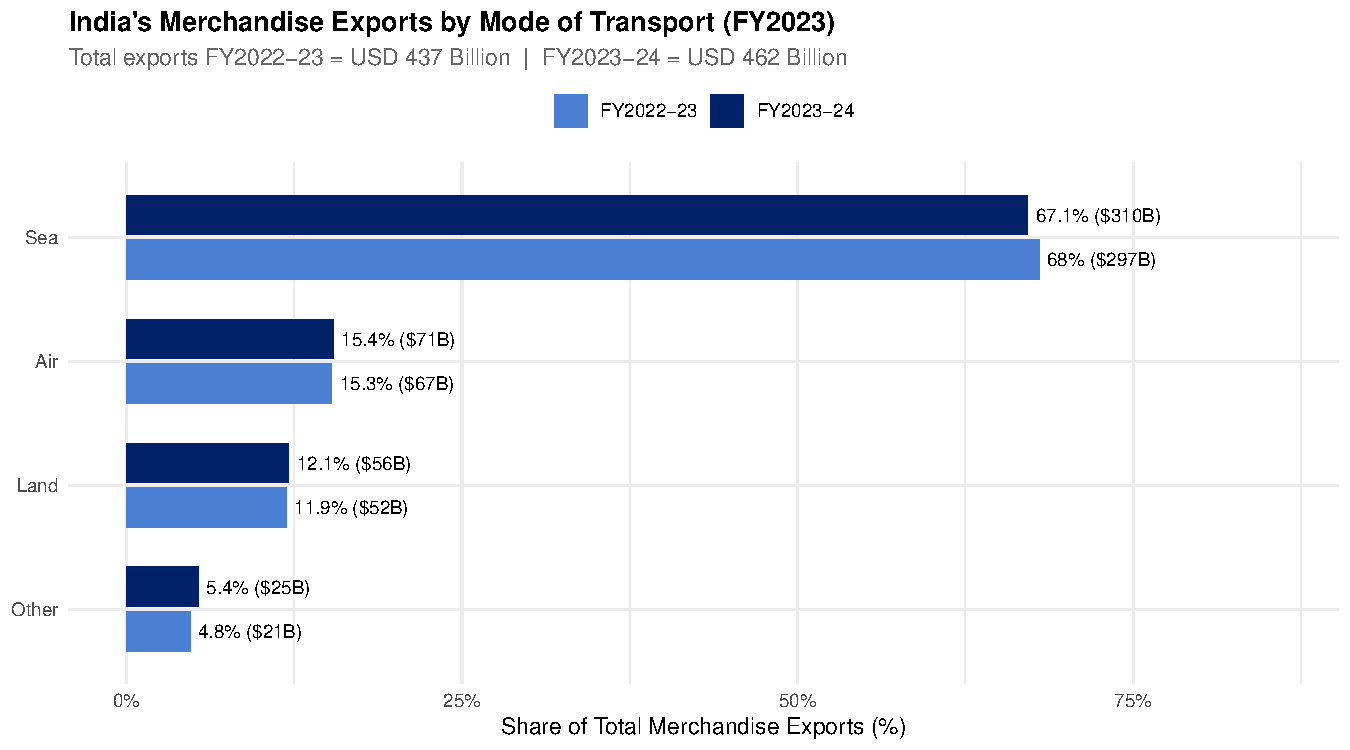
\includegraphics[keepaspectratio]{Lecture16_Export_Procedures_files/figure-beamer/fig-export-mode-1.pdf}}

}

\caption{\label{fig-export-mode}Sea freight dominates at
\textasciitilde68\% of India's merchandise exports; air
(\textasciitilde15\%) and land (\textasciitilde12\%) are secondary
modes. Share composition is stable across both years. Source: DGCI\&S /
Ministry of Commerce and Industry, GoI.}

\end{figure}%
\end{block}
\end{frame}

\begin{frame}
\begin{block}{Direct vs Indirect Export Channels}
\phantomsection\label{direct-vs-indirect-export-channels}
\begin{columns}[T]
\begin{column}{0.5\linewidth}
\textbf{Direct Export:} - Exporter deals directly with foreign buyer -
Higher margin, full control over branding/pricing - Higher risk
(counterparty, forex, compliance) - Requires: IEC, RCMC, AD bank, full
documentation - Suited to: large processors, established exporters

\textbf{Examples:} Kohinoor Foods (basmati direct to UAE retail),
Venkateshwara Hatcheries (poultry to Middle East)
\end{column}

\begin{column}{0.5\linewidth}
\textbf{Indirect Export:} - Sell to a \textbf{Merchant Exporter (ME)}
who manages the export - No direct forex exposure; simpler for small
farmer/processor - Lower price realisation (merchant takes margin) - ME
provides GST exemption on purchase from manufacturer at 0.1\% CGST+SGST

\textbf{Export Management Company (EMC):} manages exports on commission
without taking title to goods.

\textbf{FPO Route:} ::: \{.keybox\} \textbf{Farmer Producer
Organisations (FPOs)} aggregate smallholders (avg. 1.5 ha in Karnataka)
to meet minimum export quantity. APEDA's FPO Connect links 1,200+ FPOs
to export markets. Tur dal FPOs in Gulbarga district now export directly
to UK Indian grocery wholesalers.
\end{column}
\end{columns}

:::
\end{block}
\end{frame}

\begin{frame}
\begin{block}{Export Houses: India's Trade Titans}
\phantomsection\label{export-houses-indias-trade-titans}
\begin{columns}[T]
\begin{column}{0.55\linewidth}
The Government of India recognises export performance tiers with
\textbf{Star Export House} status, conferring priority clearances, bank
credit, and EPCG benefits:

\begin{longtable}[]{@{}lll@{}}
\toprule\noalign{}
Status & Min. Export (3-yr avg) & Benefits \\
\midrule\noalign{}
\endhead
Export House & ₹100 crore & Priority treatment \\
Trading House & ₹500 crore & Self-certification of CoO \\
Star Trading House & ₹2,000 crore & Fast-track customs, AEO \\
Premier Trading House & ₹10,000 crore & All of above + policy voice \\
\bottomrule\noalign{}
\end{longtable}
\end{column}

\begin{column}{0.45\linewidth}
\textbf{Major agri export houses (India):}

\begin{itemize}
\tightlist
\item
  \textbf{ITC Agribusiness:} wheat, spices, processed food; exports to
  60+ countries; \$1B+ annual turnover
\item
  \textbf{Olam International:} cashew, spices, coffee; integrated from
  farm to retail
\item
  \textbf{Adani Agri Fresh:} apple, potato, processed; cold chain
  integration
\item
  \textbf{KRBL Ltd:} world's largest basmati rice brand (India Gate);
  exports to 90+ countries
\item
  \textbf{Apex Frozen Foods:} shrimp to USA/EU; vertically integrated
  aquaculture
\end{itemize}

These firms account for \textbf{\textasciitilde35\%} of India's total
agricultural export value.
\end{column}
\end{columns}
\end{block}
\end{frame}

\begin{frame}
\begin{block}{Export Incentive Schemes}
\phantomsection\label{export-incentive-schemes}
\begin{columns}[T]
\begin{column}{0.5\linewidth}
\textbf{1. RoDTEP (Remission of Duties and Taxes on Exported Products)}
- Replaced MEIS in January 2021 (WTO-compliant) - Refunds embedded taxes
not otherwise refunded: SGST, mandi tax, electricity duty, stamp duty -
Agri rates: \textbf{0.5\% to 4.3\% of FOB value} - Issued as
transferable scrips on ICEGATE

\textbf{2. Advance Authorisation (AA)} - Duty-free import of inputs used
in export production - Standard Input Output Norms (SION) define input
ratios - Example: basmati rice exporter imports paddy from Nepal
duty-free under AA

\textbf{3. EPCG (Export Promotion Capital Goods)} - Import capital goods
(cold storage, processing equipment) at \textbf{0--3\% duty} - In
return, commit to export 6× the duty saved over 6 years
\end{column}

\begin{column}{0.5\linewidth}
\textbf{4. Transport and Marketing Assistance (TMA)} - Freight subsidy
for agri exports to notified markets (Africa, EU, USA) - Cover: 50\% of
sea freight for small exporters; 25\% for large - Products: fresh
fruits/vegetables, processed food, organic, floriculture

\textbf{5. MAI Scheme (Market Access Initiative)} - APEDA funds
participation in international trade fairs (Gulfood Dubai, SIAL Paris,
Annapoorna Mumbai) - Buyer-seller meets, market studies, reverse buyer
visits - Budget: ₹250 crore/year for all export promotion councils

\textbf{WTO compliance note:} RoDTEP is WTO-consistent (remission of
domestic taxes, not export subsidy). AA and EPCG are permissible under
WTO SCM Agreement as tax exemptions on inputs. TMA freight subsidy is
under scrutiny --- USA has raised concerns at WTO DSB.
\end{column}
\end{columns}
\end{block}
\end{frame}

\begin{frame}
\begin{block}{FSSAI and Food Safety Compliance for Exports}
\phantomsection\label{fssai-and-food-safety-compliance-for-exports}
\begin{columns}[T]
\begin{column}{0.55\linewidth}
\textbf{FSSAI (Food Safety and Standards Authority of India)}

\begin{itemize}
\tightlist
\item
  Central licensing authority for all food businesses including
  exporters
\item
  An \textbf{FSSAI Central Licence} is mandatory for
  manufacturers/processors exporting food products
\item
  Annual turnover \textgreater{} ₹20 crore or multi-state operation →
  Central Licence
\end{itemize}

\textbf{FSSAI's role in exports:}

\begin{enumerate}
\tightlist
\item
  \textbf{Standards alignment:} FSSAI standards increasingly aligned
  with Codex Alimentarius (facilitates market access)
\item
  \textbf{Organic certification:} FSSAI-accredited certification bodies
  issue Indian Organic Certificate (recognises NPOP)
\item
  \textbf{Bilateral equivalence:} FSSAI has equivalence arrangements
  with USDA NOP (organic) --- US organic certifiers can certify Indian
  organic products
\end{enumerate}
\end{column}

\begin{column}{0.45\linewidth}
\textbf{EIC accreditation for key markets:}

The \textbf{Export Inspection Council (EIC)} issues health certificates
that importing countries accept:

\begin{longtable}[]{@{}lll@{}}
\toprule\noalign{}
Market & Certificate & Requirement \\
\midrule\noalign{}
\endhead
European Union & EIC Health Cert. & Meat, fish, dairy \\
USA (FDA) & EIC + prior notice & Marine, processed \\
Japan & EIC + residue test & Marine, processed \\
Middle East & Halal + EIC & Meat, poultry \\
\bottomrule\noalign{}
\end{longtable}

EIC operates 5 regional offices (Mumbai, Chennai, Kochi, Kolkata, Delhi)
and 40 sub-offices. In FY2024, EIC certified \textbf{₹1.1 lakh crore}
worth of exports.
\end{column}
\end{columns}
\end{block}
\end{frame}

\begin{frame}{Case Study}
\phantomsection\label{case-study}
\textbf{Exporting Basmati Rice from Punjab to Saudi Arabia}

\emph{Tracing every document, agency, and payment from paddy field to
Riyadh shelf}
\end{frame}

\begin{frame}
\begin{block}{Case Study: Punjab Basmati to Saudi Arabia --- Part I}
\phantomsection\label{case-study-punjab-basmati-to-saudi-arabia-part-i}
\begin{columns}[T]
\begin{column}{0.55\linewidth}
\textbf{The exporter:} Amritsar-based rice miller; 10,000 tonne annual
capacity. Target: 500 MT to Saudi retail chain.

\textbf{Step 1 --- Registrations:} - IEC from DGFT portal (already held)
- APEDA RCMC (renewed annually; fee ₹7,500) - FSSAI Central Licence - AD
Bank: State Bank of India, Amritsar branch

\textbf{Step 2 --- Contract:} - Incoterm: \textbf{CIF Jeddah} - Price:
\$1,100/MT; Total: \$550,000 - Payment: \textbf{Sight LC} from Riyad
Bank (Saudi), advised through SBI

\textbf{Step 3 --- Procurement:} - Procures paddy from Amritsar mandi at
MSP + premium - Milling, grading, drying; APEDA quality check (aroma,
grain length)
\end{column}

\begin{column}{0.45\linewidth}
\textbf{Step 4 --- Documents prepared:}

\begin{longtable}[]{@{}lll@{}}
\toprule\noalign{}
\# & Document & Issuing Agency \\
\midrule\noalign{}
\endhead
1 & Commercial Invoice & Exporter \\
2 & Packing List & Exporter \\
3 & Certificate of Origin & FIEO/Chamber \\
4 & Phytosanitary Certificate & PPQS Punjab \\
5 & Fumigation Certificate & Licensed fumigator \\
6 & Quality/Weight Certificate & EIC / SGS \\
7 & APEDA Certificate & APEDA \\
8 & B/L & Shipping line (NSICT) \\
9 & EDPMS export declaration & RBI system (auto) \\
10 & Shipping Bill & ICEGATE (Customs) \\
\bottomrule\noalign{}
\end{longtable}
\end{column}
\end{columns}
\end{block}
\end{frame}

\begin{frame}
\begin{block}{Case Study: Punjab Basmati to Saudi Arabia --- Part II}
\phantomsection\label{case-study-punjab-basmati-to-saudi-arabia-part-ii}
\begin{columns}[T]
\begin{column}{0.55\linewidth}
\textbf{Step 5 --- Customs clearance (JNPT, Mumbai):} - Exporter files
Shipping Bill on ICEGATE: \textbf{Drawback type} (to claim duty drawback
on GST paid on packaging) - RMS assigns \textbf{Green Channel} --- LEO
granted within 3 hours - Container loaded; B/L issued by Maersk

\textbf{Step 6 --- Banking:} - Exporter presents all 10 documents to SBI
within \textbf{21 days of B/L date} (LC requirement) - SBI verifies
documents against LC terms: ✓ - SBI claims payment from Riyad Bank -
\textbf{Sight LC:} SBI receives USD 550,000 within 5 working days - SBI
converts USD to INR; credits exporter account

\textbf{Step 7 --- Post-shipment:} - RBI's EDPMS marks export as
``realised'' - Exporter files \textbf{e-BRC} (electronic Bank
Realisation Certificate) on DGFT portal - RoDTEP scrip of
\textasciitilde₹11 lakh (2\% of FOB) issued
\end{column}

\begin{column}{0.45\linewidth}
\textbf{Saudi Arabia end:}

\begin{itemize}
\tightlist
\item
  Saudi SFDA (food authority) inspects on arrival
\item
  Certificate of Origin checked against GCC preferential tariff rules
\item
  Phytosanitary certificate accepted by Saudi Plant Protection
\item
  If fumigation certificate absent → shipment quarantined
\end{itemize}

\textbf{Typical timeline (farm to Riyadh shelf):}

\begin{longtable}[]{@{}ll@{}}
\toprule\noalign{}
Stage & Days \\
\midrule\noalign{}
\endhead
Procurement + milling & 15 \\
Documentation & 5 \\
Port + customs & 3 \\
Sea transit (JNPT--Jeddah) & 8 \\
Saudi customs clearance & 5 \\
Distribution to shelf & 7 \\
\textbf{Total} & \textbf{\textasciitilde43 days} \\
\bottomrule\noalign{}
\end{longtable}
\end{column}
\end{columns}
\end{block}
\end{frame}

\begin{frame}
\begin{block}{Import Procedures: The Mirror Image}
\phantomsection\label{import-procedures-the-mirror-image}
\begin{columns}[T]
\begin{column}{0.55\linewidth}
Import procedures mirror export procedures on the buyer side.

\textbf{Key documents for agricultural imports to India:}

\begin{enumerate}
\tightlist
\item
  \textbf{Bill of Entry} --- filed on ICEGATE by importer (equivalent of
  Shipping Bill)
\item
  \textbf{Commercial Invoice and Packing List}
\item
  \textbf{Bill of Lading / Airway Bill}
\item
  \textbf{Certificate of Origin} --- for FTA preferential duty
\item
  \textbf{SPS/Phytosanitary Certificate} --- from exporting country's
  authority
\end{enumerate}

\textbf{Customs assessment:} - RMS assigns risk category - Basic Customs
Duty + IGST (at GST rate) assessed - IGST paid by importer; can claim
ITC if registered
\end{column}

\begin{column}{0.45\linewidth}
\textbf{SPS inspection for agricultural imports:}

Under the \textbf{Plant Quarantine Order 2003} and \textbf{Meat Food
Products Order}, all agri imports are subject to:

\begin{itemize}
\tightlist
\item
  Document verification (phytosanitary cert)
\item
  Physical sampling and lab testing
\item
  For pests: fumigation before release
\end{itemize}

\textbf{Restricted/Prohibited imports:}

\begin{itemize}
\tightlist
\item
  \textbf{STE channel:} wheat, rice, sugar, fertilisers --- importable
  only through state trading enterprises (FCI, NAFED, MMTC) under
  quantitative restrictions
\item
  \textbf{License required:} some oilseeds, livestock products
\item
  \textbf{Prohibited:} live pigs (several ports), certain livestock
  breeds without quarantine
\end{itemize}

\textbf{Bill of Entry types:} Home Consumption (B/E), Warehousing (W/E),
Ex-Bond (E/B).
\end{column}
\end{columns}
\end{block}
\end{frame}

\begin{frame}
\begin{block}{Logistics and Infrastructure Challenges}
\phantomsection\label{logistics-and-infrastructure-challenges}
\begin{columns}[T]
\begin{column}{0.55\linewidth}
India's \textbf{Logistics Performance Index (LPI)} rank: \textbf{38 out
of 139} (World Bank, 2023) --- up from rank 44 in 2018.

\textbf{Key bottlenecks for agricultural exports:}

\textbf{1. Port congestion:} - JNPT handles 55\% of India's container
traffic; average dwell time: \textbf{3.2 days} (global best: 1.5 days) -
Mundra, Chennai, Kochi also congested during harvest seasons

\textbf{2. Cold chain deficit:} - India's cold storage capacity:
\textbf{\textasciitilde35 million MT} (FY2024) - Requirement for
horticulture + marine: \textbf{\textasciitilde90 million MT} - Gap = 55
million MT → 25--40\% post-harvest losses in fruits and vegetables

\textbf{3. Last-mile connectivity:} - Farm-to-port road quality: NH
coverage improving, but mandi-to-cold store roads often unpaved in
Karnataka/Maharashtra
\end{column}

\begin{column}{0.45\linewidth}
\textbf{Cost of logistics as \% of GDP:}

\begin{longtable}[]{@{}ll@{}}
\toprule\noalign{}
Country & Logistics Cost / GDP \\
\midrule\noalign{}
\endhead
Germany & 8\% \\
USA & 8\% \\
China & 14\% \\
\textbf{India} & \textbf{\textasciitilde14\%} \\
\bottomrule\noalign{}
\end{longtable}

High logistics costs reduce India's price competitiveness despite low
labour costs.

\textbf{PM GatiShakti:} National Master Plan integrating roads,
railways, ports, warehouses. Target: reduce logistics cost to
\textbf{8\% of GDP by 2030}.

\textbf{Dedicated Freight Corridors (DFC):} Eastern (Ludhiana--Kolkata)
and Western (JNPT--Dadri) operational 2024 --- will cut rail freight
time by 40\% for Punjab basmati, Maharashtra grapes.
\end{column}
\end{columns}
\end{block}
\end{frame}

\begin{frame}
\begin{block}{Digital Initiatives in Export Trade}
\phantomsection\label{digital-initiatives-in-export-trade}
\begin{columns}[T]
\begin{column}{0.55\linewidth}
\textbf{DGFT Digital Modernisation (2021--ongoing):}

\begin{itemize}
\tightlist
\item
  Fully online IEC issuance: \textbf{24 hours} (was 3 weeks paper-based)
\item
  Online RCMC by APEDA: auto-linked to IEC
\item
  e-BRC (electronic Bank Realisation Certificate): exporter's bank
  submits directly to DGFT portal; no paper filing
\item
  \textbf{DARPAN platform:} dashboard for tracking all incentive scheme
  status in real time
\end{itemize}

\textbf{SWIFT (Single Window Interface for Facilitating Trade):} - One
portal for customs, FSSAI, PPQS, Drug Controller, textile ministry
clearances - Launched 2016; covers 26 regulatory agencies - 2024
expansion: includes MPEDA, APEDA certificates integrated
\end{column}

\begin{column}{0.45\linewidth}
\textbf{ICEGATE 2.0 (launched 2023):}

\begin{itemize}
\tightlist
\item
  AI-based risk management system → 70\% of shipments now on Green
  Channel (was 55\%)
\item
  e-Sanchit: paperless document upload --- all 10 export documents can
  be uploaded digitally; customs officer reviews on-screen
\item
  Integration with GSTN: automatic input tax credit verification for
  RoDTEP computation
\end{itemize}

\textbf{APEDA-DGFT integration:}

APEDA's NHB system auto-generates RCMC data to DGFT; exporters need not
re-enter. Certificate of Origin auto-populated from ICEGATE data for FTA
claims.

India's trade facilitation score (WTO TFA): \textbf{90.59\%} (2023) ---
above developing-country average of 74\%.
\end{column}
\end{columns}
\end{block}
\end{frame}

\begin{frame}[fragile]
\begin{block}{Summary: The Export Ecosystem}
\phantomsection\label{summary-the-export-ecosystem}
\begin{columns}[T]
\begin{column}{0.55\linewidth}
\textbf{The full export chain for Indian agri:}

\begin{verbatim}
Farmer/Processor
      ↓ FPO aggregation / merchant exporter
IEC + RCMC + FSSAI + AD Bank
      ↓ pre-shipment
Export Contract (Incoterm negotiated)
      ↓ finance
Letter of Credit (bank guarantee)
      ↓ documentation
10 documents (Invoice, B/L, CoO, Phyto, EIC...)
      ↓ customs
ICEGATE Shipping Bill → LEO
      ↓ logistics
Port → Ship → Destination customs
      ↓ payment
Bank realises forex → e-BRC filed
      ↓ incentives
RoDTEP scrip + drawback + TMA
\end{verbatim}
\end{column}

\begin{column}{0.45\linewidth}
\textbf{Key Takeaways:}

\begin{enumerate}
\tightlist
\item
  \textbf{IEC is the master key} --- no export without it
\item
  \textbf{The Shipping Bill + LEO} is the customs clearance milestone
  --- nothing loads without it
\item
  \textbf{The Bill of Lading} is the only negotiable title document ---
  it unlocks payment under LC
\item
  \textbf{RoDTEP} has replaced MEIS as the primary export incentive ---
  WTO-compliant, duty refund basis
\item
  \textbf{Cold chain and logistics} remain India's primary structural
  bottleneck --- world-class documentation systems exist, but physical
  infrastructure lags
\item
  \textbf{Digital India} is working: ICEGATE, SWIFT, e-BRC have
  dramatically reduced transaction costs
\end{enumerate}
\end{column}
\end{columns}
\end{block}
\end{frame}

\begin{frame}
\begin{block}{Next Lecture}
\phantomsection\label{next-lecture}
\textbf{Lecture 17 --- Agricultural Export Promotion Organizations}\\
\emph{August 15, 2026}

\begin{itemize}
\tightlist
\item
  APEDA: mandate, functions, financial assistance, market access
  achievements
\item
  MPEDA and India's \$7.6 billion seafood export ecosystem
\item
  The five Commodity Boards: Tea, Coffee, Rubber, Spices, Tobacco
\item
  Export Inspection Council and quality certification
\item
  NAFED: buffer stocks, MSP procurement, export implications
\item
  Farmer Producer Organizations as export units
\item
  India's 2030 export target: \$60 billion in agri and food products
\end{itemize}

\textbf{Preparation:} Review APEDA Annual Report 2023--24 (available at
apeda.gov.in). Note the top 10 products by export value and the top 5
destination countries.
\end{block}
\end{frame}

\begin{frame}{Appendix}
\phantomsection\label{appendix}
\begin{block}{Additional Resources}
\phantomsection\label{additional-resources}
\begin{columns}[T]
\begin{column}{0.5\linewidth}
\textbf{Further Reading}

\begin{itemize}
\tightlist
\item
  Lecture notes and APEDA/WTO official documents
\item
  DGFT: Foreign Trade Policy 2023-28
\item
  RBI/DGCI\&S/APEDA databases for latest data
\end{itemize}
\end{column}

\begin{column}{0.5\linewidth}
\textbf{Key Data Sources}

\begin{itemize}
\tightlist
\item
  DGCI\&S: India's merchandise trade
\item
  RBI: Balance of payments data\\
\item
  APEDA: Agricultural export statistics
\item
  WTO: Tariff and trade databases
\end{itemize}
\end{column}
\end{columns}
\end{block}
\end{frame}




\end{document}
